% Options for packages loaded elsewhere
\PassOptionsToPackage{unicode}{hyperref}
\PassOptionsToPackage{hyphens}{url}
%
\documentclass[
]{article}
\usepackage{lmodern}
\usepackage{amssymb,amsmath}
\usepackage{ifxetex,ifluatex}
\ifnum 0\ifxetex 1\fi\ifluatex 1\fi=0 % if pdftex
  \usepackage[T1]{fontenc}
  \usepackage[utf8]{inputenc}
  \usepackage{textcomp} % provide euro and other symbols
\else % if luatex or xetex
  \usepackage{unicode-math}
  \defaultfontfeatures{Scale=MatchLowercase}
  \defaultfontfeatures[\rmfamily]{Ligatures=TeX,Scale=1}
\fi
% Use upquote if available, for straight quotes in verbatim environments
\IfFileExists{upquote.sty}{\usepackage{upquote}}{}
\IfFileExists{microtype.sty}{% use microtype if available
  \usepackage[]{microtype}
  \UseMicrotypeSet[protrusion]{basicmath} % disable protrusion for tt fonts
}{}
\makeatletter
\@ifundefined{KOMAClassName}{% if non-KOMA class
  \IfFileExists{parskip.sty}{%
    \usepackage{parskip}
  }{% else
    \setlength{\parindent}{0pt}
    \setlength{\parskip}{6pt plus 2pt minus 1pt}}
}{% if KOMA class
  \KOMAoptions{parskip=half}}
\makeatother
\usepackage{xcolor}
\IfFileExists{xurl.sty}{\usepackage{xurl}}{} % add URL line breaks if available
\IfFileExists{bookmark.sty}{\usepackage{bookmark}}{\usepackage{hyperref}}
\hypersetup{
  pdftitle={FIMSummary},
  pdfauthor={Manuel Alcalá Kovalski},
  hidelinks,
  pdfcreator={LaTeX via pandoc}}
\urlstyle{same} % disable monospaced font for URLs
\usepackage[margin=1in]{geometry}
\usepackage{graphicx}
\makeatletter
\def\maxwidth{\ifdim\Gin@nat@width>\linewidth\linewidth\else\Gin@nat@width\fi}
\def\maxheight{\ifdim\Gin@nat@height>\textheight\textheight\else\Gin@nat@height\fi}
\makeatother
% Scale images if necessary, so that they will not overflow the page
% margins by default, and it is still possible to overwrite the defaults
% using explicit options in \includegraphics[width, height, ...]{}
\setkeys{Gin}{width=\maxwidth,height=\maxheight,keepaspectratio}
% Set default figure placement to htbp
\makeatletter
\def\fps@figure{htbp}
\makeatother
\setlength{\emergencystretch}{3em} % prevent overfull lines
\providecommand{\tightlist}{%
  \setlength{\itemsep}{0pt}\setlength{\parskip}{0pt}}
\setcounter{secnumdepth}{-\maxdimen} % remove section numbering
\ifluatex
  \usepackage{selnolig}  % disable illegal ligatures
\fi

\title{FIMSummary}
\author{Manuel Alcalá Kovalski}
\date{10/16/2020}

\begin{document}
\maketitle

\begin{verbatim}
## Warning: package 'tidyverse' was built under R version 4.0.2
\end{verbatim}

\begin{verbatim}
## Warning: package 'ggplot2' was built under R version 4.0.2
\end{verbatim}

\begin{verbatim}
## Warning: package 'tibble' was built under R version 4.0.2
\end{verbatim}

\begin{verbatim}
## Warning: package 'tidyr' was built under R version 4.0.2
\end{verbatim}

\begin{verbatim}
## Warning: package 'readr' was built under R version 4.0.2
\end{verbatim}

\begin{verbatim}
## Warning: package 'purrr' was built under R version 4.0.2
\end{verbatim}

\begin{verbatim}
## Warning: package 'dplyr' was built under R version 4.0.2
\end{verbatim}

\begin{verbatim}
## Warning: package 'stringr' was built under R version 4.0.2
\end{verbatim}

\begin{verbatim}
## Warning: package 'forcats' was built under R version 4.0.2
\end{verbatim}

\begin{verbatim}
## Warning: package 'reshape2' was built under R version 4.0.2
\end{verbatim}

\begin{verbatim}
## Warning: package 'zoo' was built under R version 4.0.2
\end{verbatim}

\begin{verbatim}
## Warning: package 'quantmod' was built under R version 4.0.2
\end{verbatim}

\begin{verbatim}
## Warning: package 'xts' was built under R version 4.0.2
\end{verbatim}

\begin{verbatim}
## Warning: package 'TTR' was built under R version 4.0.2
\end{verbatim}

\begin{verbatim}
## Warning: package 'data.table' was built under R version 4.0.2
\end{verbatim}

\begin{verbatim}
## Warning: package 'lubridate' was built under R version 4.0.2
\end{verbatim}

\begin{verbatim}
## Warning: package 'Hmisc' was built under R version 4.0.2
\end{verbatim}

\begin{verbatim}
## Warning: package 'survival' was built under R version 4.0.2
\end{verbatim}

\begin{verbatim}
## Warning: package 'magrittr' was built under R version 4.0.2
\end{verbatim}

\begin{verbatim}
## Warning: package 'readxl' was built under R version 4.0.2
\end{verbatim}

\begin{verbatim}
## Warning: package 'writexl' was built under R version 4.0.2
\end{verbatim}

\begin{verbatim}
## Warning: package 'ggthemes' was built under R version 4.0.2
\end{verbatim}

\begin{verbatim}
## Warning: package 'ggtext' was built under R version 4.0.2
\end{verbatim}

\begin{verbatim}
## Warning: package 'gridExtra' was built under R version 4.0.2
\end{verbatim}

\begin{verbatim}
## Warning: package 'wesanderson' was built under R version 4.0.2
\end{verbatim}

\begin{verbatim}
## Warning: package 'tinytex' was built under R version 4.0.2
\end{verbatim}

\begin{verbatim}
## Warning: Missing column names filled in: 'X1' [1]

## Warning: Missing column names filled in: 'X1' [1]
\end{verbatim}

\begin{verbatim}
## Warning: The `x` argument of `as_tibble()` can't be missing as of lifecycle 3.0.0.
## This warning is displayed once every 8 hours.
## Call `lifecycle::last_warnings()` to see where this warning was generated.
\end{verbatim}

\begin{verbatim}
## Warning: Missing column names filled in: 'X1' [1]
\end{verbatim}

\begin{verbatim}
## Warning in mask$eval_all_filter(dots, env_filter): Incompatible methods
## (">.Date", "Ops.data.frame") for ">"
\end{verbatim}

\begin{verbatim}
## Warning: Problem with `mutate()` input `..1`.
## i Incompatible methods (">=.Date", "Ops.data.frame") for ">="
## i Input `..1` is `across(...)`.
\end{verbatim}

\begin{verbatim}
## Warning in if_else(date >= mpc_lag & date <= Q4_2021,
## mpc_health_outlays_CRN19(.x), : Incompatible methods (">=.Date",
## "Ops.data.frame") for ">="
\end{verbatim}

\begin{verbatim}
## Warning: Problem with `mutate()` input `..1`.
## i Incompatible methods (">=.Date", "Ops.data.frame") for ">="
## i Input `..1` is `across(...)`.
\end{verbatim}

\begin{verbatim}
## Warning in if_else(date >= mpc_lag & date <= Q4_2021,
## mpc_health_outlays_CRN19(.x), : Incompatible methods (">=.Date",
## "Ops.data.frame") for ">="
\end{verbatim}

\begin{verbatim}
## Warning: Problem with `mutate()` input `..1`.
## i Incompatible methods (">=.Date", "Ops.data.frame") for ">="
## i Input `..1` is `across(...)`.
\end{verbatim}

\begin{verbatim}
## Warning in if_else(date >= mpc_lag & date <= Q4_2021,
## mpc_health_outlays_CRN19(.x), : Incompatible methods (">=.Date",
## "Ops.data.frame") for ">="
\end{verbatim}

\begin{verbatim}
## Warning: Problem with `mutate()` input `..1`.
## i Incompatible methods (">=.Date", "Ops.data.frame") for ">="
## i Input `..1` is `across(...)`.
\end{verbatim}

\begin{verbatim}
## Warning in if_else(date >= mpc_lag & date <= Q4_2021,
## mpc_social_benefits_CRN19(.x), : Incompatible methods (">=.Date",
## "Ops.data.frame") for ">="
\end{verbatim}

\begin{verbatim}
## Warning: Problem with `mutate()` input `..1`.
## i Incompatible methods (">=.Date", "Ops.data.frame") for ">="
## i Input `..1` is `across(...)`.
\end{verbatim}

\begin{verbatim}
## Warning in if_else(date >= mpc_lag & date <= Q4_2021,
## mpc_social_benefits_CRN19(.x), : Incompatible methods (">=.Date",
## "Ops.data.frame") for ">="
\end{verbatim}

\begin{verbatim}
## Warning: Problem with `mutate()` input `..1`.
## i Incompatible methods (">=.Date", "Ops.data.frame") for ">="
## i Input `..1` is `across(...)`.
\end{verbatim}

\begin{verbatim}
## Warning in if_else(date >= mpc_lag & date <= Q4_2021,
## mpc_social_benefits_CRN19(.x), : Incompatible methods (">=.Date",
## "Ops.data.frame") for ">="
\end{verbatim}

\begin{verbatim}
## Warning: Problem with `mutate()` input `..1`.
## i Incompatible methods (">=.Date", "Ops.data.frame") for ">="
## i Input `..1` is `across(...)`.
\end{verbatim}

\begin{verbatim}
## Warning in if_else(date >= mpc_lag & date <= Q4_2021,
## mpc_corporate_taxes_CRN19(.x), : Incompatible methods (">=.Date",
## "Ops.data.frame") for ">="
\end{verbatim}

\begin{verbatim}
## Warning: Problem with `mutate()` input `..1`.
## i Incompatible methods (">=.Date", "Ops.data.frame") for ">="
## i Input `..1` is `across(...)`.
\end{verbatim}

\begin{verbatim}
## Warning in if_else(date >= mpc_lag & date <= Q4_2021,
## mpc_corporate_taxes_CRN19(.x), : Incompatible methods (">=.Date",
## "Ops.data.frame") for ">="
\end{verbatim}

\begin{verbatim}
## Warning: Problem with `mutate()` input `..1`.
## i Incompatible methods (">=.Date", "Ops.data.frame") for ">="
## i Input `..1` is `across(...)`.
\end{verbatim}

\begin{verbatim}
## Warning in if_else(date >= mpc_lag & date <= Q4_2021,
## mpc_corporate_taxes_CRN19(.x), : Incompatible methods (">=.Date",
## "Ops.data.frame") for ">="
\end{verbatim}

\begin{verbatim}
## Warning: Problem with `mutate()` input `..1`.
## i Incompatible methods (">=.Date", "Ops.data.frame") for ">="
## i Input `..1` is `across(...)`.
\end{verbatim}

\begin{verbatim}
## Warning in if_else(date >= mpc_lag & date <= Q4_2021,
## mpc_noncorp_taxes_CRN19(.x), : Incompatible methods (">=.Date",
## "Ops.data.frame") for ">="
\end{verbatim}

\begin{verbatim}
## Warning: Problem with `mutate()` input `..1`.
## i Incompatible methods (">=.Date", "Ops.data.frame") for ">="
## i Input `..1` is `across(...)`.
\end{verbatim}

\begin{verbatim}
## Warning in if_else(date >= mpc_lag & date <= Q4_2021,
## mpc_noncorp_taxes_CRN19(.x), : Incompatible methods (">=.Date",
## "Ops.data.frame") for ">="
\end{verbatim}

\begin{verbatim}
## Warning: Problem with `mutate()` input `..1`.
## i Incompatible methods (">=.Date", "Ops.data.frame") for ">="
## i Input `..1` is `across(...)`.
\end{verbatim}

\begin{verbatim}
## Warning in if_else(date >= mpc_lag & date <= Q4_2021,
## mpc_noncorp_taxes_CRN19(.x), : Incompatible methods (">=.Date",
## "Ops.data.frame") for ">="
\end{verbatim}

\begin{verbatim}
## Warning: Problem with `mutate()` input `..1`.
## i Incompatible methods (">=.Date", "Ops.data.frame") for ">="
## i Input `..1` is `across(...)`.
\end{verbatim}

\begin{verbatim}
## Warning in if_else(date >= mpc_lag & date <= Q4_2021, mpc_subsidies(.x), :
## Incompatible methods (">=.Date", "Ops.data.frame") for ">="
\end{verbatim}

\begin{verbatim}
## Warning: Problem with `mutate()` input `..1`.
## i Incompatible methods (">=.Date", "Ops.data.frame") for ">="
## i Input `..1` is `across(...)`.
\end{verbatim}

\begin{verbatim}
## Warning in if_else(date >= mpc_lag & date <= Q4_2021, mpc_subsidies(.x), :
## Incompatible methods (">=.Date", "Ops.data.frame") for ">="
\end{verbatim}

\begin{verbatim}
## Warning: Problem with `mutate()` input `..1`.
## i Incompatible methods (">=.Date", "Ops.data.frame") for ">="
## i Input `..1` is `across(...)`.
\end{verbatim}

\begin{verbatim}
## Warning in if_else(date >= mpc_lag & date <= Q4_2021, mpc_subsidies(.x), :
## Incompatible methods (">=.Date", "Ops.data.frame") for ">="
\end{verbatim}

\hypertarget{components}{%
\subsection{Components}\label{components}}

Our quarterly fiscal impact measure is:

\[FIM_{t} = FIM^{Fed}_{t} + FIM^{S \&L}_{t}  + FIM^{Taxes \ \& \ Transfers}  \]

\begin{center}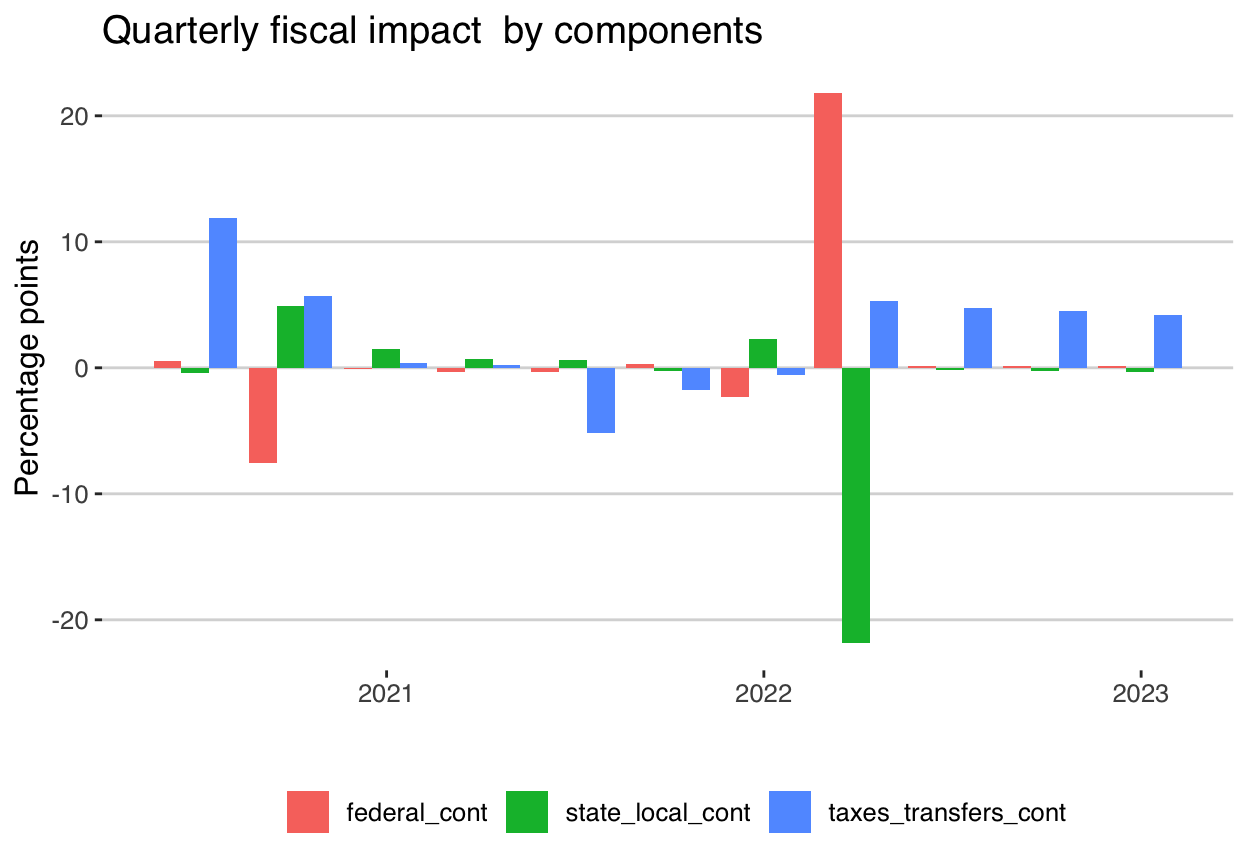
\includegraphics{summary_files/figure-latex/bars-1} \end{center}

\hypertarget{federal-purchases}{%
\subsubsection{Federal purchases}\label{federal-purchases}}

The contribution of federal purchases is the sum of the contributions of
federal spending, consumption grants, and investment grants to GDP.

\[FIM^{Fed,\ Purchases}_{t} = FIM^{Fed,\ Spending}_{t} + FIM^{Fed, \ Consumption\ Grants}_{t} + FIM^{Fed, \ Investment\ Grants}_{t} \]

\begin{center}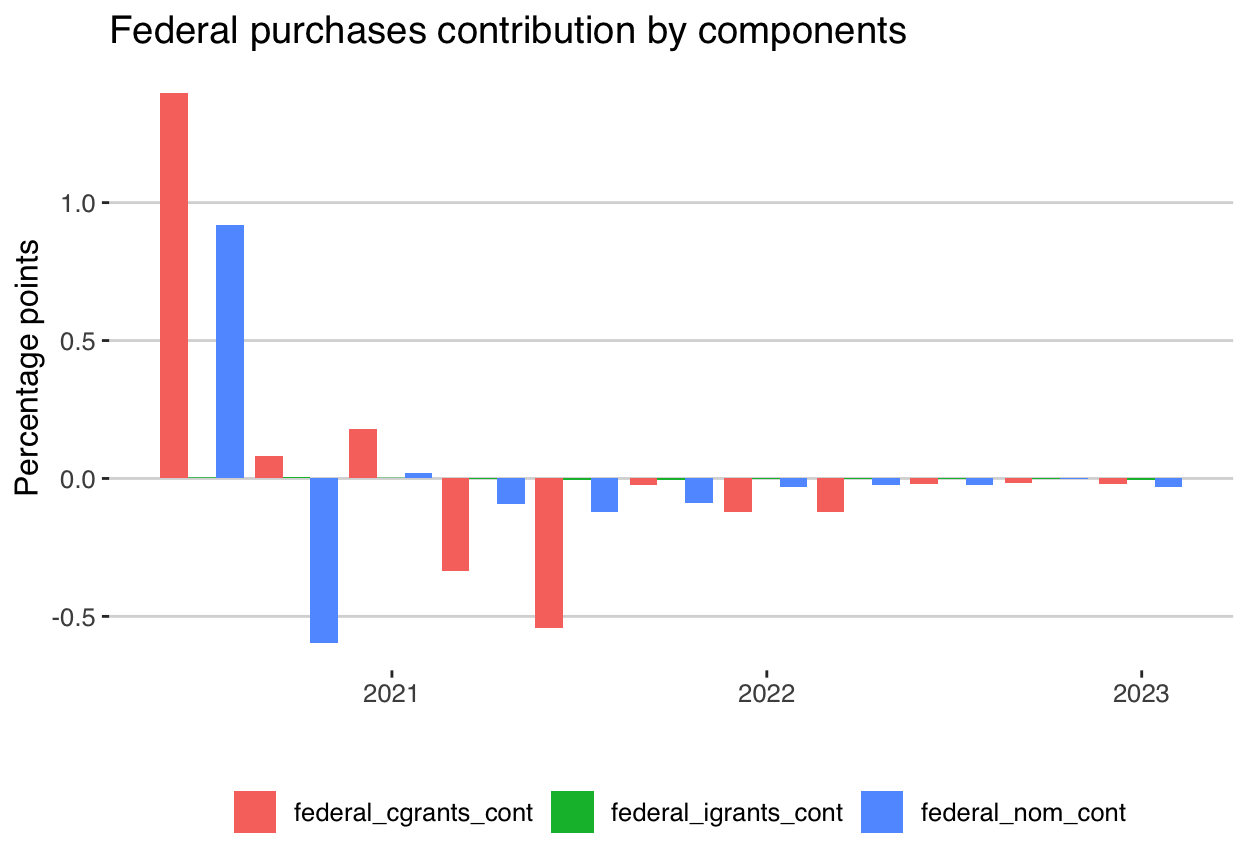
\includegraphics{summary_files/figure-latex/federal purchases-1} \end{center}

\hypertarget{state-purchases}{%
\subsubsection{State purchases}\label{state-purchases}}

Similarily, the contribution of state \& local purchases is the sum of
the contributions of State \& Local spending minus consumption grants,
and investment grants to GDP. That is,

\[FIM^{S\&L,\  Purchases}_{t} = FIM^{S\&L,\ Spending}_{t} - FIM^{Fed,\ Consumption\ Grants}_{t} - FIM^{Fed,\ Investment\ Grants}_{t} \]

\begin{center}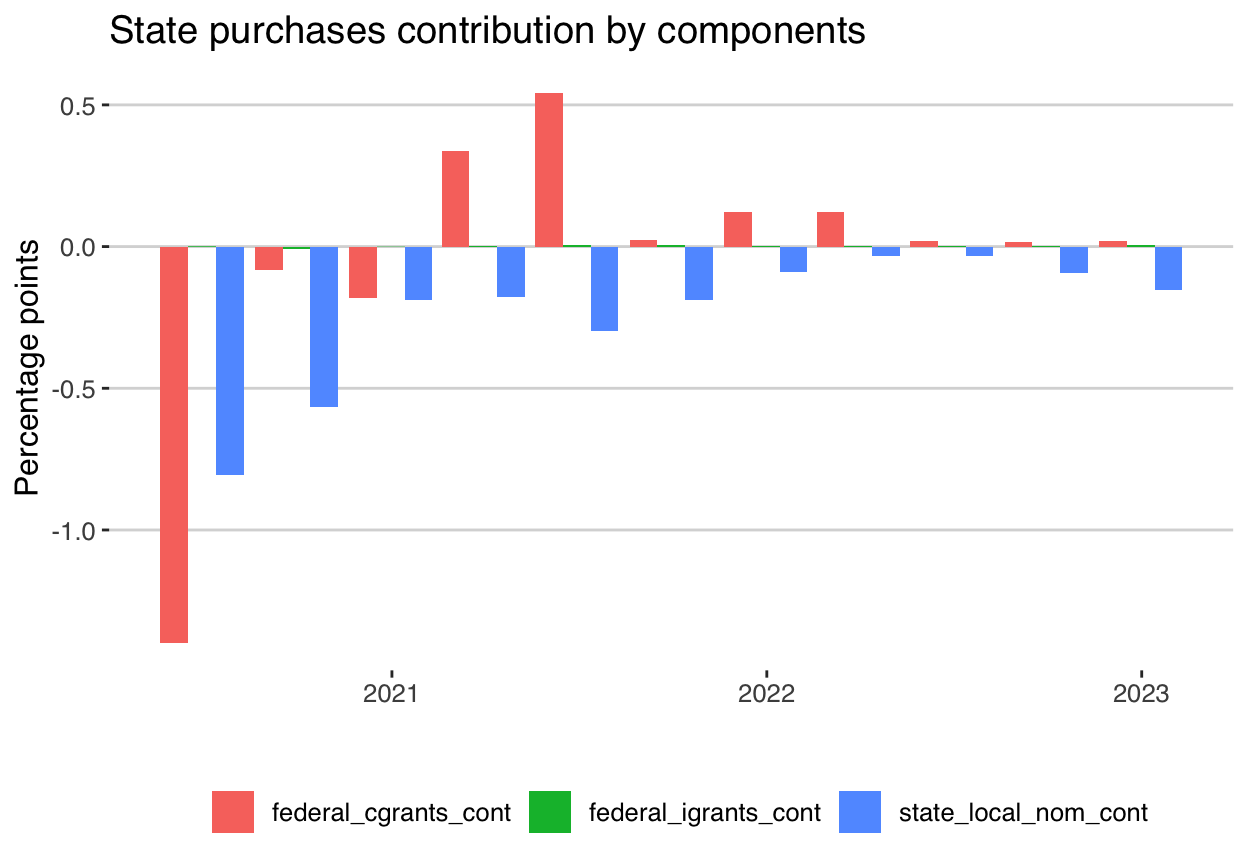
\includegraphics{summary_files/figure-latex/state purchases-1} \end{center}

The pieces used to calculate these contributions were nominal federal
and S\&L spending, federal consumption grants, and investment grants.
Federal consumption grants consist of federal consumption grants to
state net of Medicaid grants.

\begin{center}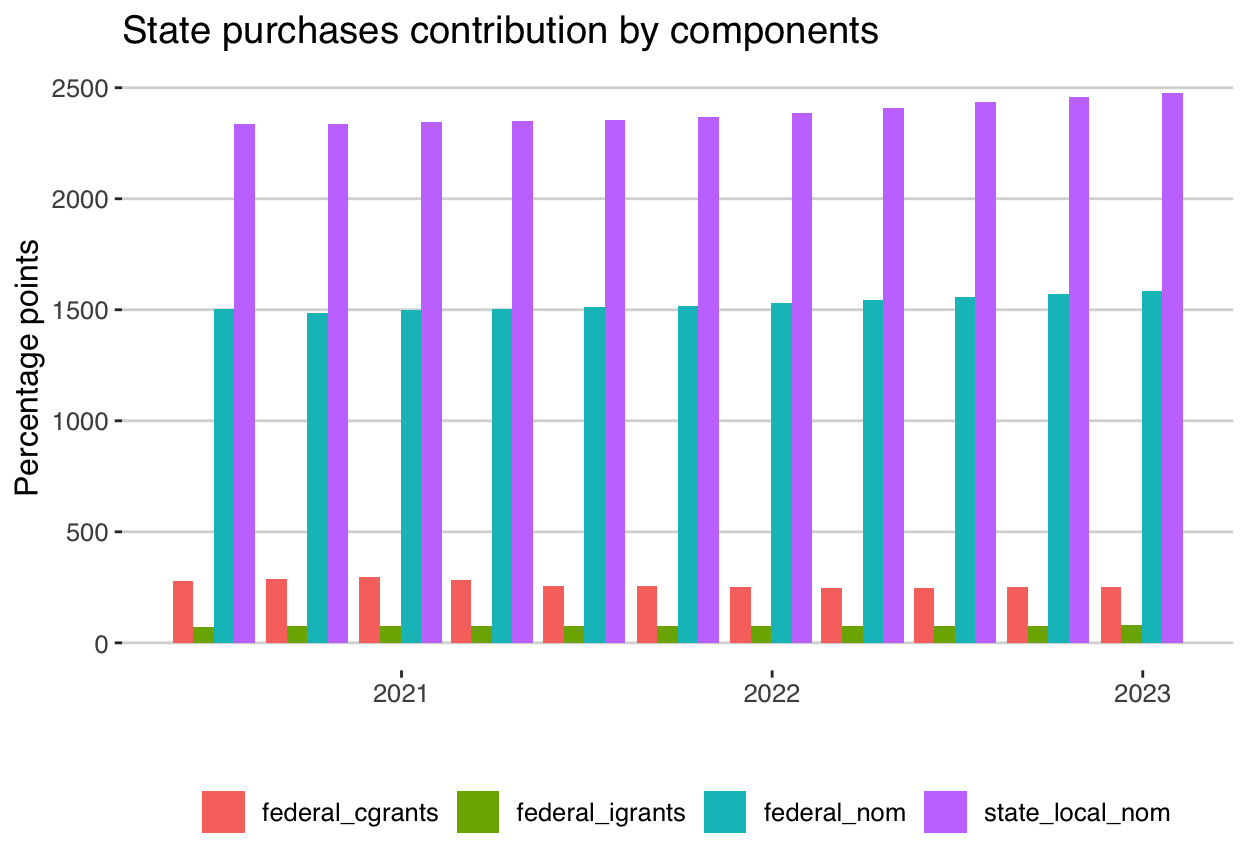
\includegraphics{summary_files/figure-latex/purchases pieces-1} \end{center}

To understand the level of our federal cgrants we must know the levels
for gross consumption grants, medicaid grants, health and hospital
grants. Because of COVID legislation, we also need to know our add
factor for net consumption grants.

\begin{center}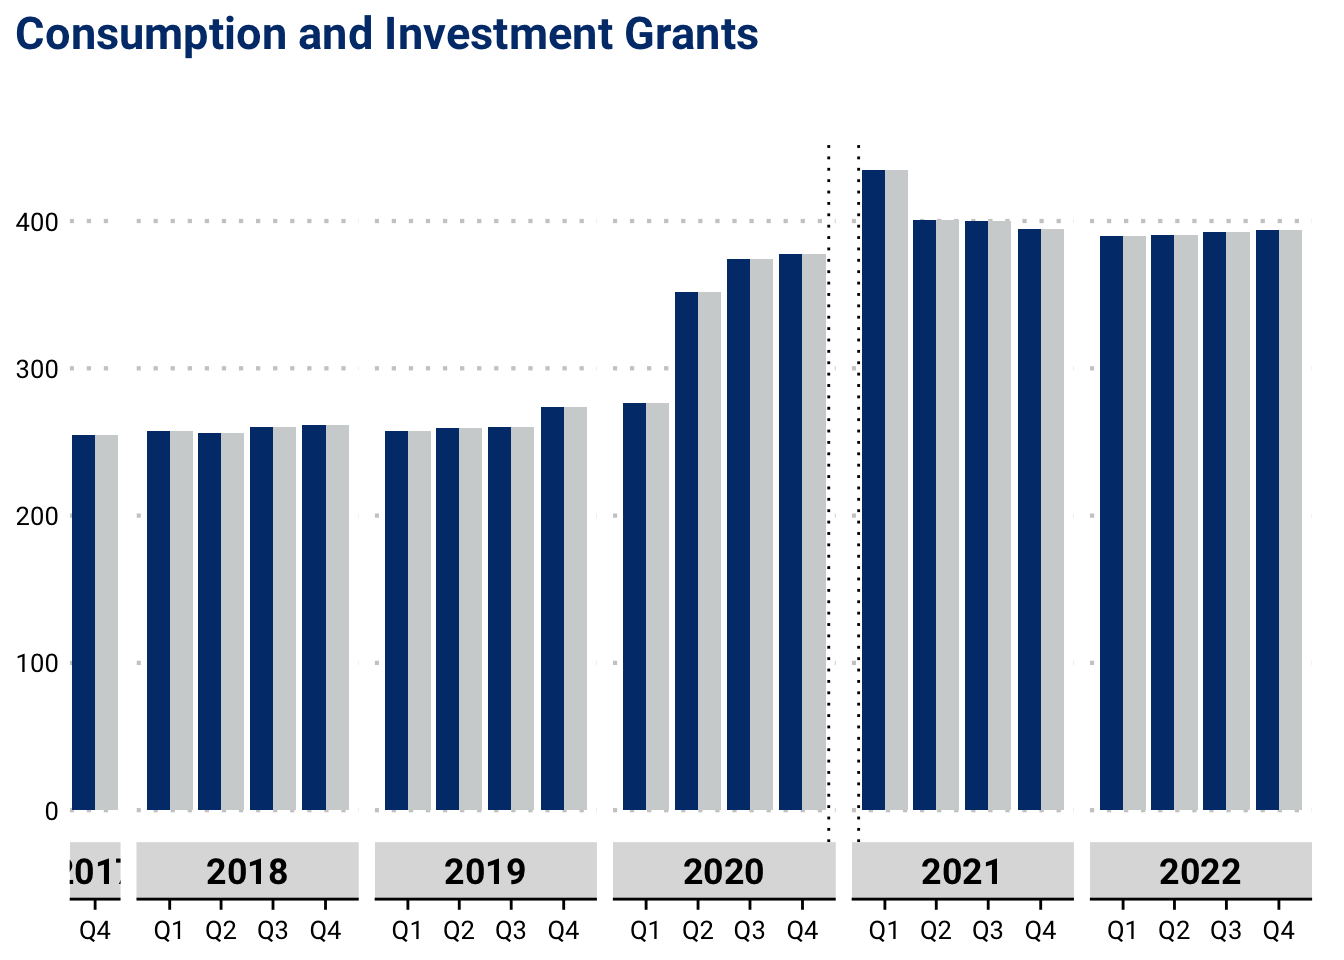
\includegraphics{summary_files/figure-latex/unnamed-chunk-2-1} \end{center}

\hypertarget{taxes-transfers-and-subsidies}{%
\subsubsection{Taxes, transfers and
subsidies}\label{taxes-transfers-and-subsidies}}

\[FIM^{Taxes\ \& \ Transfers} = FIM^{Taxes\ \&\ Transfers} + FIM^{Subsidies}  \]

\begin{center}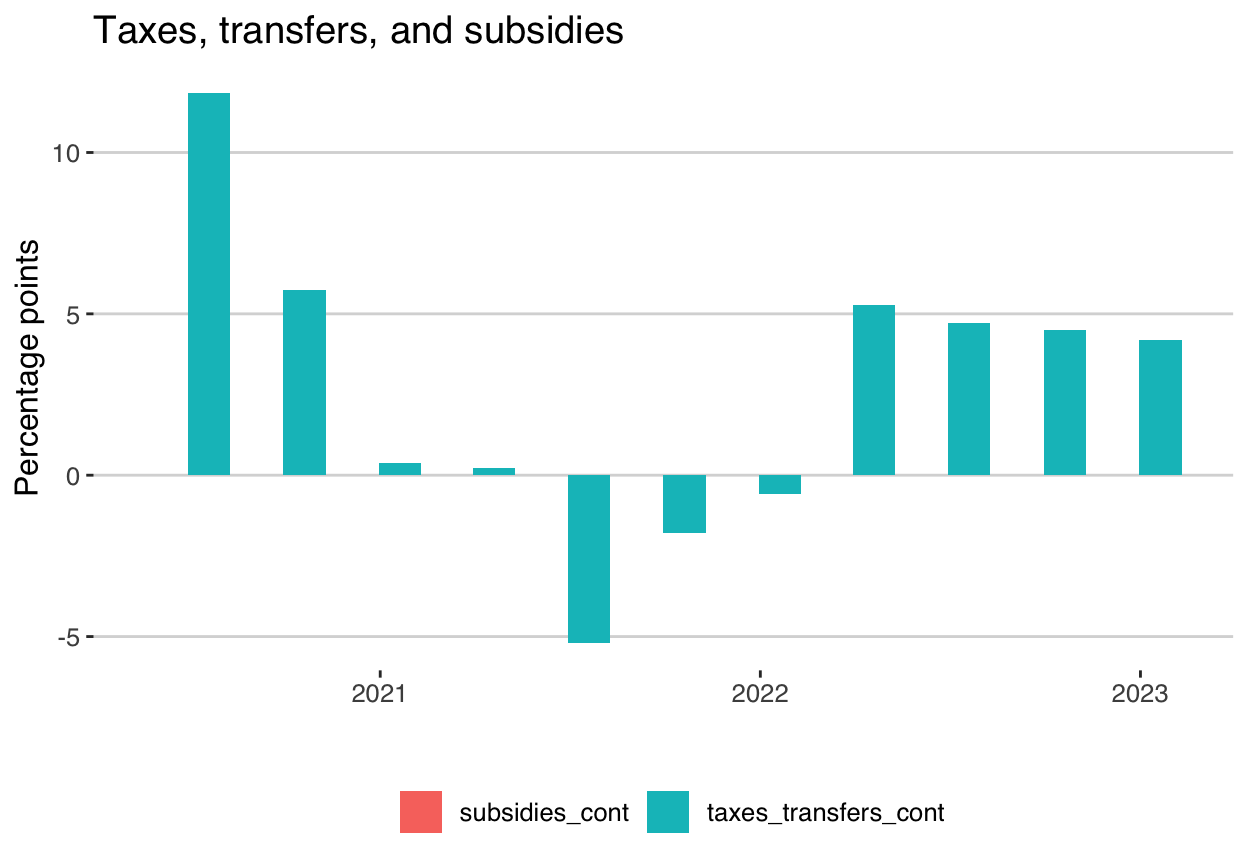
\includegraphics{summary_files/figure-latex/taxes transfers and subsidies-1} \end{center}

\hypertarget{taxes-transfers-subsidies-by-level-of-government}{%
\subsection{Taxes, transfers, subsidies by level of
government}\label{taxes-transfers-subsidies-by-level-of-government}}

\hypertarget{government-taxes}{%
\subsubsection{Government Taxes}\label{government-taxes}}

\begin{center}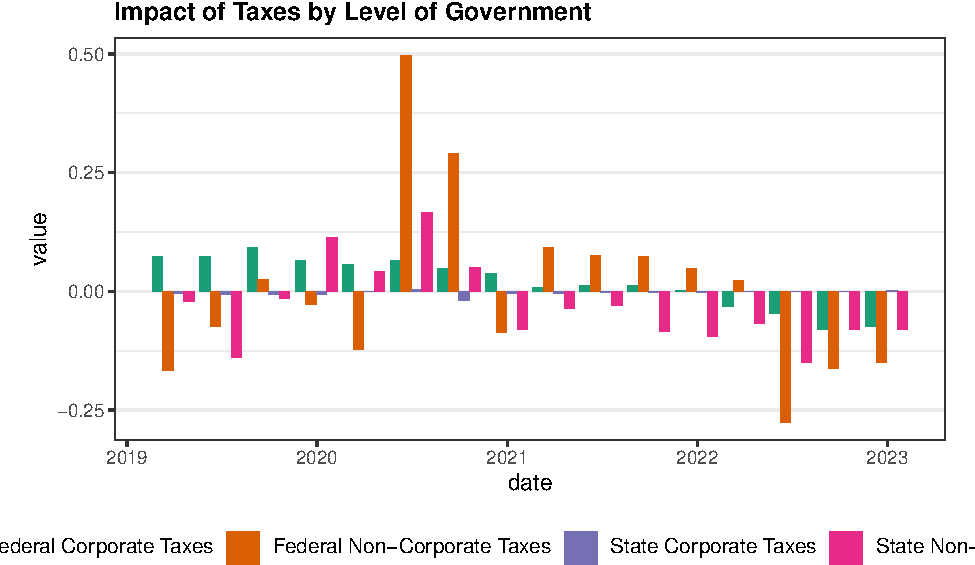
\includegraphics{summary_files/figure-latex/taxes-1} \end{center}

\hypertarget{federal-taxes}{%
\subsubsection{Federal Taxes}\label{federal-taxes}}

\begin{center}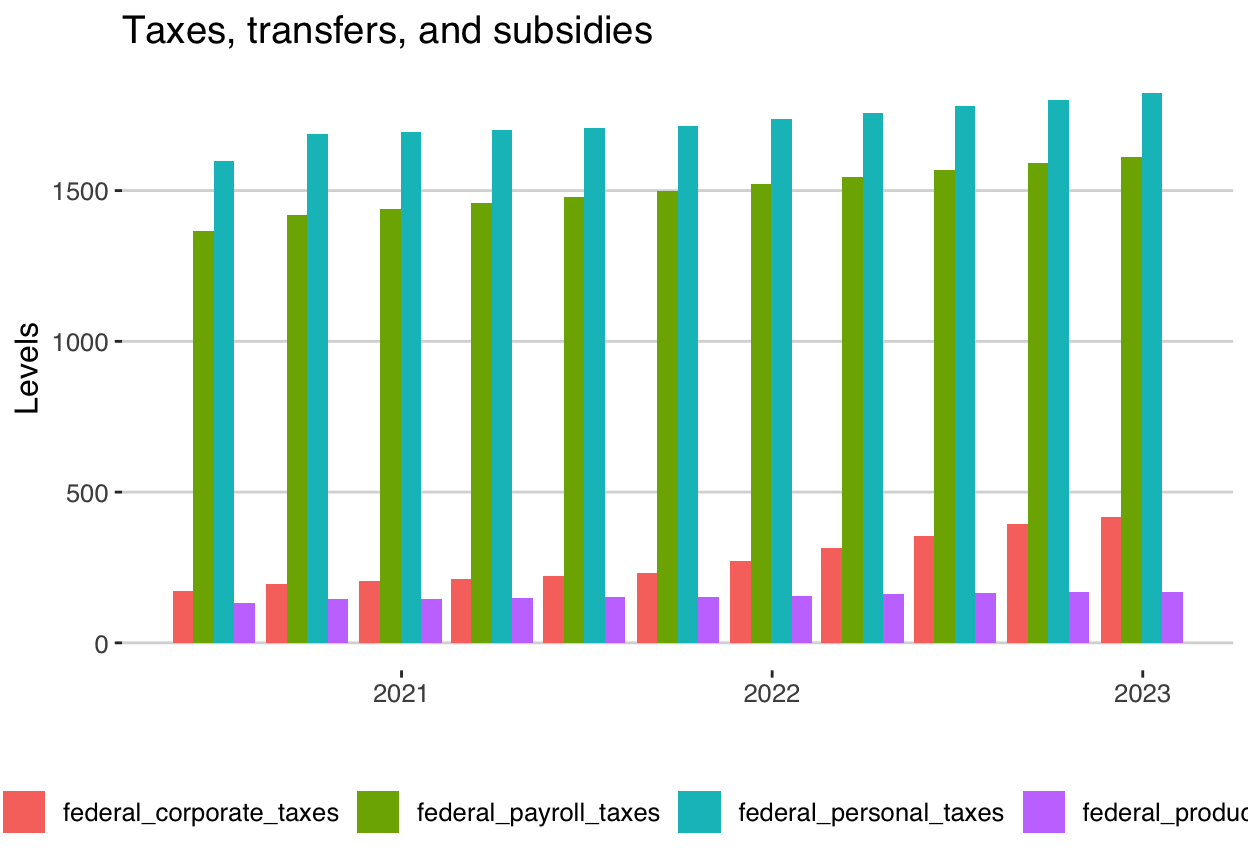
\includegraphics{summary_files/figure-latex/federal taxes-1} \end{center}

\hypertarget{state-local-taxes}{%
\subsubsection{State \& Local Taxes}\label{state-local-taxes}}

\begin{center}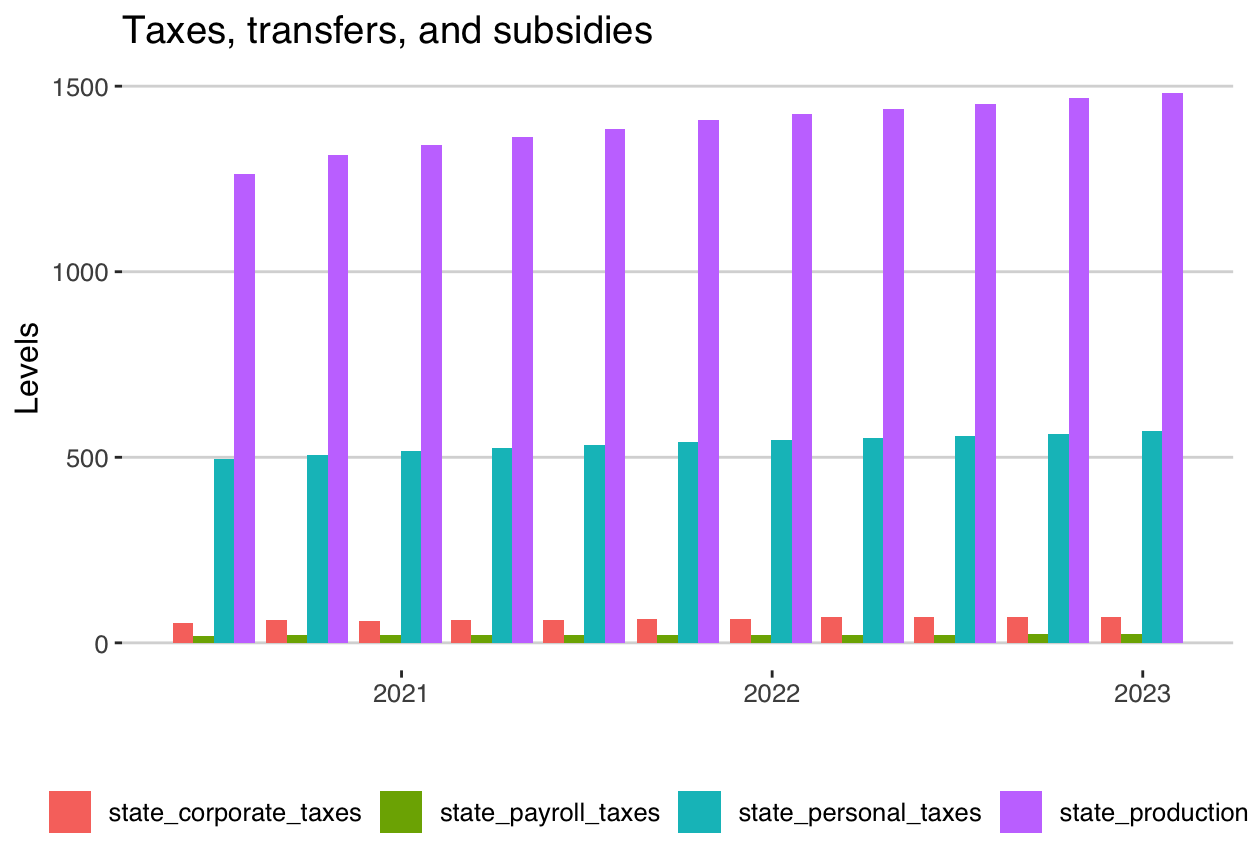
\includegraphics{summary_files/figure-latex/state taxes-1} \end{center}

\hypertarget{government-transfers}{%
\subsubsection{Government Transfers}\label{government-transfers}}

\begin{center}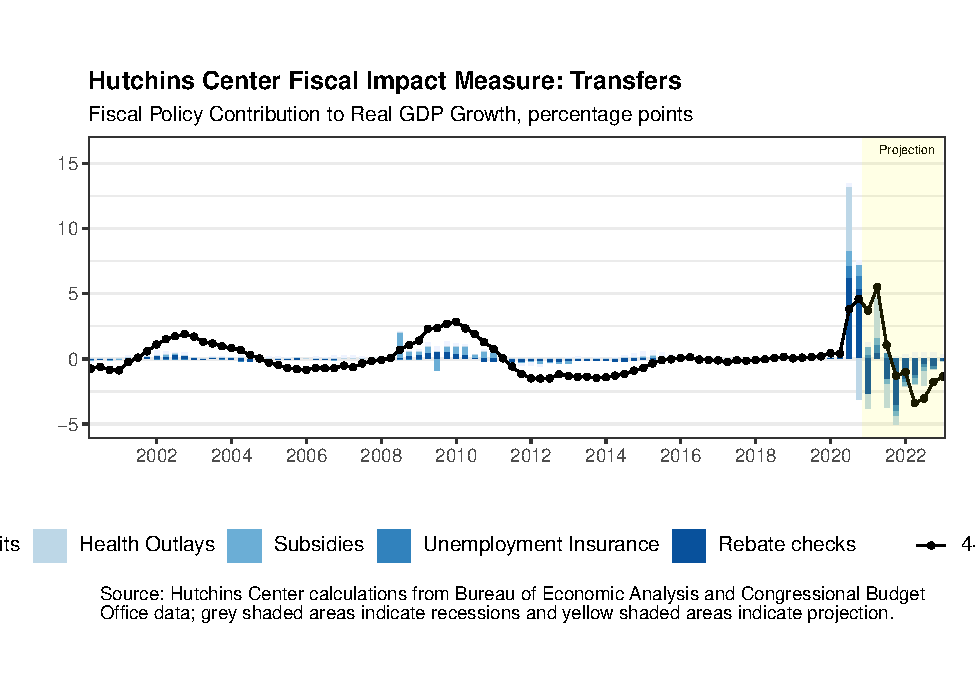
\includegraphics{summary_files/figure-latex/transfers-1} \end{center}

\hypertarget{subsidies}{%
\subsubsection{Subsidies}\label{subsidies}}

\begin{center}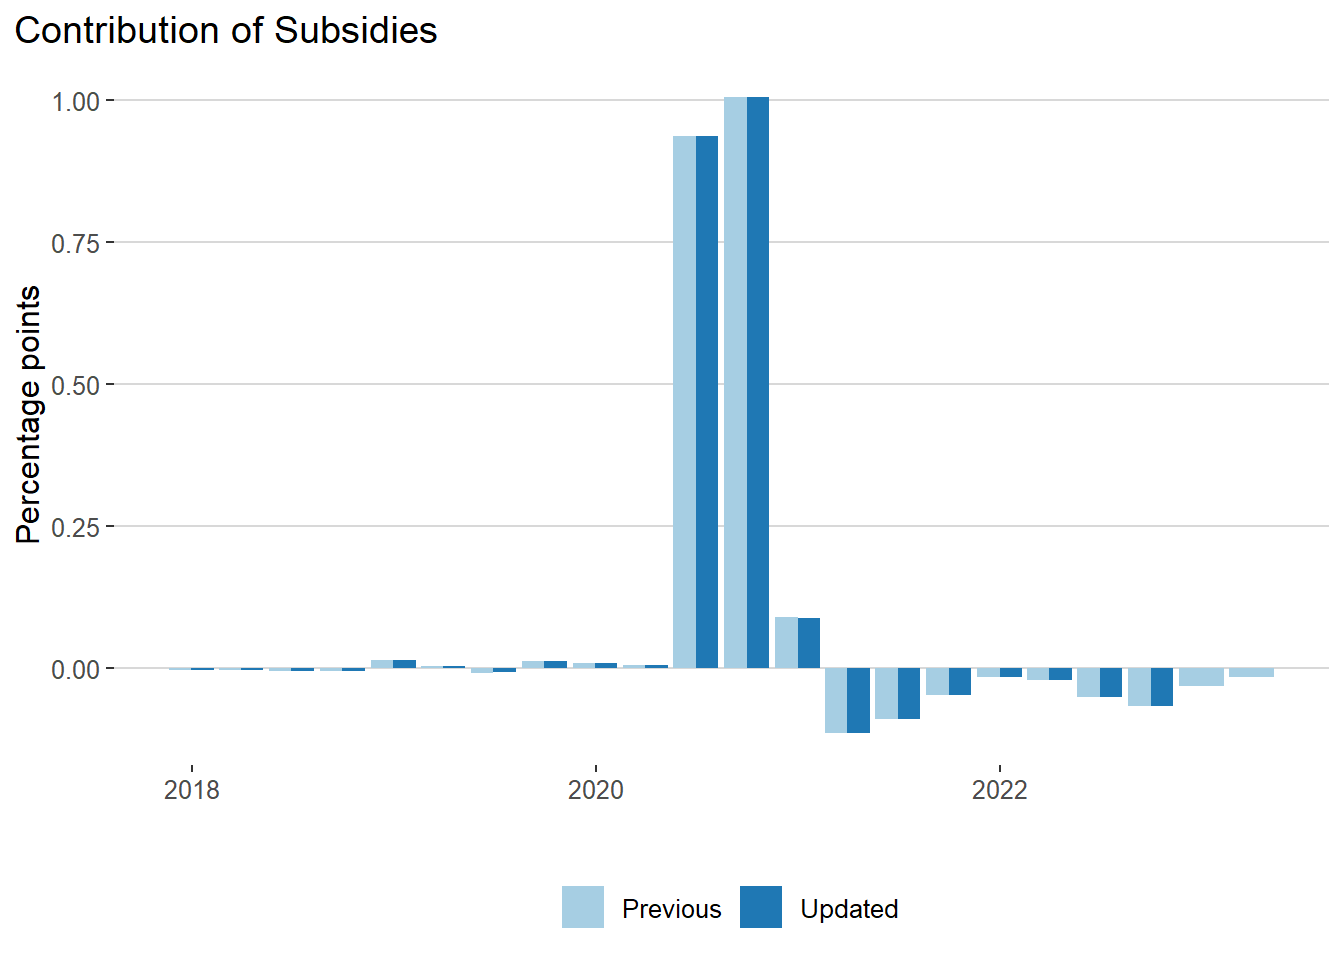
\includegraphics{summary_files/figure-latex/subsidies-1} \end{center}

\end{document}
